\documentclass[twoside]{book}

% Packages required by doxygen
\usepackage{calc}
\usepackage{doxygen}
\usepackage{graphicx}
\usepackage[utf8]{inputenc}
\usepackage{makeidx}
\usepackage{multicol}
\usepackage{multirow}
\usepackage{textcomp}
\usepackage[table]{xcolor}

% Font selection
\usepackage[T1]{fontenc}
\usepackage{mathptmx}
\usepackage[scaled=.90]{helvet}
\usepackage{courier}
\usepackage{amssymb}
\usepackage{sectsty}
\renewcommand{\familydefault}{\sfdefault}
\allsectionsfont{%
  \fontseries{bc}\selectfont%
  \color{darkgray}%
}
\renewcommand{\DoxyLabelFont}{%
  \fontseries{bc}\selectfont%
  \color{darkgray}%
}

% Page & text layout
\usepackage{geometry}
\geometry{%
  a4paper,%
  top=2.5cm,%
  bottom=2.5cm,%
  left=2.5cm,%
  right=2.5cm%
}
\tolerance=750
\hfuzz=15pt
\hbadness=750
\setlength{\emergencystretch}{15pt}
\setlength{\parindent}{0cm}
\setlength{\parskip}{0.2cm}
\makeatletter
\renewcommand{\paragraph}{%
  \@startsection{paragraph}{4}{0ex}{-1.0ex}{1.0ex}{%
    \normalfont\normalsize\bfseries\SS@parafont%
  }%
}
\renewcommand{\subparagraph}{%
  \@startsection{subparagraph}{5}{0ex}{-1.0ex}{1.0ex}{%
    \normalfont\normalsize\bfseries\SS@subparafont%
  }%
}
\makeatother

% Headers & footers
\usepackage{fancyhdr}
\pagestyle{fancyplain}
\fancyhead[LE]{\fancyplain{}{\bfseries\thepage}}
\fancyhead[CE]{\fancyplain{}{}}
\fancyhead[RE]{\fancyplain{}{\bfseries\leftmark}}
\fancyhead[LO]{\fancyplain{}{\bfseries\rightmark}}
\fancyhead[CO]{\fancyplain{}{}}
\fancyhead[RO]{\fancyplain{}{\bfseries\thepage}}
\fancyfoot[LE]{\fancyplain{}{}}
\fancyfoot[CE]{\fancyplain{}{}}
\fancyfoot[RE]{\fancyplain{}{\bfseries\scriptsize Generated on Sun Mar 18 2018 05\-:16\-:45 for My Project by Doxygen }}
\fancyfoot[LO]{\fancyplain{}{\bfseries\scriptsize Generated on Sun Mar 18 2018 05\-:16\-:45 for My Project by Doxygen }}
\fancyfoot[CO]{\fancyplain{}{}}
\fancyfoot[RO]{\fancyplain{}{}}
\renewcommand{\footrulewidth}{0.4pt}
\renewcommand{\chaptermark}[1]{%
  \markboth{#1}{}%
}
\renewcommand{\sectionmark}[1]{%
  \markright{\thesection\ #1}%
}

% Indices & bibliography
\usepackage{natbib}
\usepackage[titles]{tocloft}
\setcounter{tocdepth}{3}
\setcounter{secnumdepth}{5}
\makeindex

% Hyperlinks (required, but should be loaded last)
\usepackage{ifpdf}
\ifpdf
  \usepackage[pdftex,pagebackref=true]{hyperref}
\else
  \usepackage[ps2pdf,pagebackref=true]{hyperref}
\fi
\hypersetup{%
  colorlinks=true,%
  linkcolor=blue,%
  citecolor=blue,%
  unicode%
}

% Custom commands
\newcommand{\clearemptydoublepage}{%
  \newpage{\pagestyle{empty}\cleardoublepage}%
}


%===== C O N T E N T S =====

\begin{document}

% Titlepage & ToC
\hypersetup{pageanchor=false}
\pagenumbering{roman}
\begin{titlepage}
\vspace*{7cm}
\begin{center}%
{\Large My Project }\\
\vspace*{1cm}
{\large Generated by Doxygen 1.8.6}\\
\vspace*{0.5cm}
{\small Sun Mar 18 2018 05:16:45}\\
\end{center}
\end{titlepage}
\clearemptydoublepage
\tableofcontents
\clearemptydoublepage
\pagenumbering{arabic}
\hypersetup{pageanchor=true}

%--- Begin generated contents ---
\chapter{Class Index}
\section{Class List}
Here are the classes, structs, unions and interfaces with brief descriptions\-:\begin{DoxyCompactList}
\item\contentsline{section}{\hyperlink{struct_tuple_printer}{Tuple\-Printer$<$ Tuple, N $>$} }{\pageref{struct_tuple_printer}}{}
\item\contentsline{section}{\hyperlink{struct_tuple_printer_3_01_tuple_00_011_01_4}{Tuple\-Printer$<$ Tuple, 1 $>$} }{\pageref{struct_tuple_printer_3_01_tuple_00_011_01_4}}{}
\end{DoxyCompactList}

\chapter{File Index}
\section{File List}
Here is a list of all files with brief descriptions\-:\begin{DoxyCompactList}
\item\contentsline{section}{\hyperlink{print__ip_8cpp}{print\-\_\-ip.\-cpp} }{\pageref{print__ip_8cpp}}{}
\item\contentsline{section}{\hyperlink{version_8h}{version.\-h} }{\pageref{version_8h}}{}
\end{DoxyCompactList}

\chapter{Class Documentation}
\hypertarget{struct_tuple_printer}{\section{Tuple\-Printer$<$ Tuple, N $>$ Struct Template Reference}
\label{struct_tuple_printer}\index{Tuple\-Printer$<$ Tuple, N $>$@{Tuple\-Printer$<$ Tuple, N $>$}}
}
\subsection*{Static Public Member Functions}
\begin{DoxyCompactItemize}
\item 
static void \hyperlink{struct_tuple_printer_aaf76573f278205ba63759d5dbe3f408c}{print} (const Tuple \&t)
\end{DoxyCompactItemize}


\subsection{Member Function Documentation}
\hypertarget{struct_tuple_printer_aaf76573f278205ba63759d5dbe3f408c}{\index{Tuple\-Printer@{Tuple\-Printer}!print@{print}}
\index{print@{print}!TuplePrinter@{Tuple\-Printer}}
\subsubsection[{print}]{\setlength{\rightskip}{0pt plus 5cm}template$<$typename Tuple , std\-::size\-\_\-t N$>$ static void {\bf Tuple\-Printer}$<$ Tuple, N $>$\-::print (
\begin{DoxyParamCaption}
\item[{const Tuple \&}]{t}
\end{DoxyParamCaption}
)\hspace{0.3cm}{\ttfamily [inline]}, {\ttfamily [static]}}}\label{struct_tuple_printer_aaf76573f278205ba63759d5dbe3f408c}


The documentation for this struct was generated from the following file\-:\begin{DoxyCompactItemize}
\item 
\hyperlink{print__ip_8cpp}{print\-\_\-ip.\-cpp}\end{DoxyCompactItemize}

\hypertarget{struct_tuple_printer_3_01_tuple_00_011_01_4}{\section{Tuple\-Printer$<$ Tuple, 1 $>$ Struct Template Reference}
\label{struct_tuple_printer_3_01_tuple_00_011_01_4}\index{Tuple\-Printer$<$ Tuple, 1 $>$@{Tuple\-Printer$<$ Tuple, 1 $>$}}
}
\subsection*{Static Public Member Functions}
\begin{DoxyCompactItemize}
\item 
static void \hyperlink{struct_tuple_printer_3_01_tuple_00_011_01_4_af4ab0b518a1d2927e949c817aa6b7266}{print} (const Tuple \&t)
\end{DoxyCompactItemize}


\subsection{Member Function Documentation}
\hypertarget{struct_tuple_printer_3_01_tuple_00_011_01_4_af4ab0b518a1d2927e949c817aa6b7266}{\index{Tuple\-Printer$<$ Tuple, 1 $>$@{Tuple\-Printer$<$ Tuple, 1 $>$}!print@{print}}
\index{print@{print}!TuplePrinter< Tuple, 1 >@{Tuple\-Printer$<$ Tuple, 1 $>$}}
\subsubsection[{print}]{\setlength{\rightskip}{0pt plus 5cm}template$<$typename Tuple $>$ static void {\bf Tuple\-Printer}$<$ Tuple, 1 $>$\-::print (
\begin{DoxyParamCaption}
\item[{const Tuple \&}]{t}
\end{DoxyParamCaption}
)\hspace{0.3cm}{\ttfamily [inline]}, {\ttfamily [static]}}}\label{struct_tuple_printer_3_01_tuple_00_011_01_4_af4ab0b518a1d2927e949c817aa6b7266}


The documentation for this struct was generated from the following file\-:\begin{DoxyCompactItemize}
\item 
\hyperlink{print__ip_8cpp}{print\-\_\-ip.\-cpp}\end{DoxyCompactItemize}

\chapter{File Documentation}
\hypertarget{print__ip_8cpp}{\section{print\-\_\-ip.\-cpp File Reference}
\label{print__ip_8cpp}\index{print\-\_\-ip.\-cpp@{print\-\_\-ip.\-cpp}}
}
{\ttfamily \#include $<$iostream$>$}\\*
{\ttfamily \#include $<$list$>$}\\*
{\ttfamily \#include $<$vector$>$}\\*
{\ttfamily \#include $<$string$>$}\\*
{\ttfamily \#include $<$tuple$>$}\\*
{\ttfamily \#include $<$type\-\_\-traits$>$}\\*
Include dependency graph for print\-\_\-ip.\-cpp\-:
\nopagebreak
\begin{figure}[H]
\begin{center}
\leavevmode
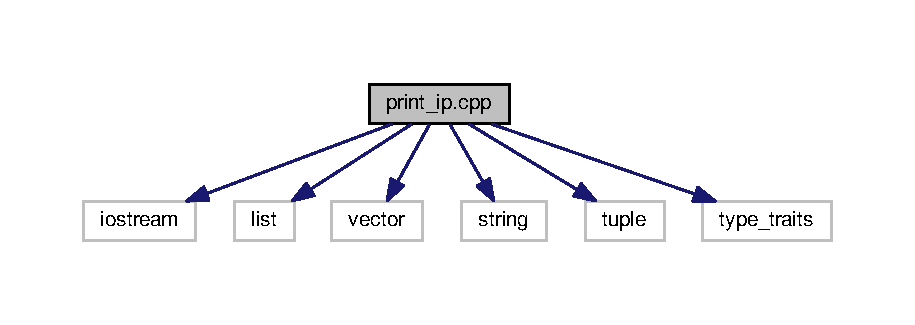
\includegraphics[width=350pt]{print__ip_8cpp__incl}
\end{center}
\end{figure}
\subsection*{Classes}
\begin{DoxyCompactItemize}
\item 
struct \hyperlink{struct_tuple_printer}{Tuple\-Printer$<$ Tuple, N $>$}
\item 
struct \hyperlink{struct_tuple_printer_3_01_tuple_00_011_01_4}{Tuple\-Printer$<$ Tuple, 1 $>$}
\end{DoxyCompactItemize}
\subsection*{Functions}
\begin{DoxyCompactItemize}
\item 
{\footnotesize template$<$typename T , typename std\-::enable\-\_\-if$<$ !(std\-::is\-\_\-integral$<$ T $>$\-::value$\vert$$\vert$std\-::is\-\_\-same$<$ T, std\-::string $>$\-::value), T $\ast$ $>$\-::type  = nullptr$>$ }\\void \hyperlink{print__ip_8cpp_add22f80e675a041f07648b701fc81b88}{print} (const T \&val)
\begin{DoxyCompactList}\small\item\em Функция печати адреса для контейнеров \end{DoxyCompactList}\item 
{\footnotesize template$<$typename T , typename std\-::enable\-\_\-if$<$ std\-::is\-\_\-integral$<$ T $>$\-::value, T $\ast$ $>$\-::type  = nullptr$>$ }\\void \hyperlink{print__ip_8cpp_ab0ee94f0f283926675c2820c1e63c9e3}{print} (T val)
\begin{DoxyCompactList}\small\item\em Функция печати адреса для целочисленных типов \end{DoxyCompactList}\item 
{\footnotesize template$<$class... Args$>$ }\\void \hyperlink{print__ip_8cpp_abe476df5eb88070c1cacb35714a8a93a}{print} (std\-::tuple$<$ Args...$>$ t)
\begin{DoxyCompactList}\small\item\em Функция печати адреса для кортежей \end{DoxyCompactList}\item 
int \hyperlink{print__ip_8cpp_ae66f6b31b5ad750f1fe042a706a4e3d4}{main} ()
\end{DoxyCompactItemize}


\subsection{Function Documentation}
\hypertarget{print__ip_8cpp_ae66f6b31b5ad750f1fe042a706a4e3d4}{\index{print\-\_\-ip.\-cpp@{print\-\_\-ip.\-cpp}!main@{main}}
\index{main@{main}!print_ip.cpp@{print\-\_\-ip.\-cpp}}
\subsubsection[{main}]{\setlength{\rightskip}{0pt plus 5cm}int main (
\begin{DoxyParamCaption}
{}
\end{DoxyParamCaption}
)}}\label{print__ip_8cpp_ae66f6b31b5ad750f1fe042a706a4e3d4}
\hypertarget{print__ip_8cpp_add22f80e675a041f07648b701fc81b88}{\index{print\-\_\-ip.\-cpp@{print\-\_\-ip.\-cpp}!print@{print}}
\index{print@{print}!print_ip.cpp@{print\-\_\-ip.\-cpp}}
\subsubsection[{print}]{\setlength{\rightskip}{0pt plus 5cm}template$<$typename T , typename std\-::enable\-\_\-if$<$ !(std\-::is\-\_\-integral$<$ T $>$\-::value$\vert$$\vert$std\-::is\-\_\-same$<$ T, std\-::string $>$\-::value), T $\ast$ $>$\-::type  = nullptr$>$ void print (
\begin{DoxyParamCaption}
\item[{const T \&}]{val}
\end{DoxyParamCaption}
)}}\label{print__ip_8cpp_add22f80e675a041f07648b701fc81b88}


Функция печати адреса для контейнеров 

Функция печати адреса для строки \hypertarget{print__ip_8cpp_ab0ee94f0f283926675c2820c1e63c9e3}{\index{print\-\_\-ip.\-cpp@{print\-\_\-ip.\-cpp}!print@{print}}
\index{print@{print}!print_ip.cpp@{print\-\_\-ip.\-cpp}}
\subsubsection[{print}]{\setlength{\rightskip}{0pt plus 5cm}template$<$typename T , typename std\-::enable\-\_\-if$<$ std\-::is\-\_\-integral$<$ T $>$\-::value, T $\ast$ $>$\-::type  = nullptr$>$ void print (
\begin{DoxyParamCaption}
\item[{T}]{val}
\end{DoxyParamCaption}
)}}\label{print__ip_8cpp_ab0ee94f0f283926675c2820c1e63c9e3}


Функция печати адреса для целочисленных типов 

\hypertarget{print__ip_8cpp_abe476df5eb88070c1cacb35714a8a93a}{\index{print\-\_\-ip.\-cpp@{print\-\_\-ip.\-cpp}!print@{print}}
\index{print@{print}!print_ip.cpp@{print\-\_\-ip.\-cpp}}
\subsubsection[{print}]{\setlength{\rightskip}{0pt plus 5cm}template$<$class... Args$>$ void print (
\begin{DoxyParamCaption}
\item[{std\-::tuple$<$ Args...$>$}]{t}
\end{DoxyParamCaption}
)}}\label{print__ip_8cpp_abe476df5eb88070c1cacb35714a8a93a}


Функция печати адреса для кортежей 


\hypertarget{version_8h}{\section{version.\-h File Reference}
\label{version_8h}\index{version.\-h@{version.\-h}}
}
\subsection*{Macros}
\begin{DoxyCompactItemize}
\item 
\#define \hyperlink{version_8h_a4a5fc96a4bdd7d68ed99ccce9ca2e77e}{P\-R\-O\-J\-E\-C\-T\-\_\-\-V\-E\-R\-S\-I\-O\-N\-\_\-\-P\-A\-T\-C\-H}~4
\end{DoxyCompactItemize}


\subsection{Macro Definition Documentation}
\hypertarget{version_8h_a4a5fc96a4bdd7d68ed99ccce9ca2e77e}{\index{version.\-h@{version.\-h}!P\-R\-O\-J\-E\-C\-T\-\_\-\-V\-E\-R\-S\-I\-O\-N\-\_\-\-P\-A\-T\-C\-H@{P\-R\-O\-J\-E\-C\-T\-\_\-\-V\-E\-R\-S\-I\-O\-N\-\_\-\-P\-A\-T\-C\-H}}
\index{P\-R\-O\-J\-E\-C\-T\-\_\-\-V\-E\-R\-S\-I\-O\-N\-\_\-\-P\-A\-T\-C\-H@{P\-R\-O\-J\-E\-C\-T\-\_\-\-V\-E\-R\-S\-I\-O\-N\-\_\-\-P\-A\-T\-C\-H}!version.h@{version.\-h}}
\subsubsection[{P\-R\-O\-J\-E\-C\-T\-\_\-\-V\-E\-R\-S\-I\-O\-N\-\_\-\-P\-A\-T\-C\-H}]{\setlength{\rightskip}{0pt plus 5cm}\#define P\-R\-O\-J\-E\-C\-T\-\_\-\-V\-E\-R\-S\-I\-O\-N\-\_\-\-P\-A\-T\-C\-H~4}}\label{version_8h_a4a5fc96a4bdd7d68ed99ccce9ca2e77e}

%--- End generated contents ---

% Index
\newpage
\phantomsection
\addcontentsline{toc}{chapter}{Index}
\printindex

\end{document}
